\documentclass{article}
\usepackage{amsmath}
\usepackage{amssymb}
\usepackage{enumitem}
\usepackage{graphicx}
\usepackage[margin=1in]{geometry}
\usepackage[overload]{empheq}
\usepackage{subcaption}
\usepackage{listings}
\usepackage{color}

% These two lines are from this StackExchange post: https://tex.stackexchange.com/a/177270
\usepackage{sectsty}
\allsectionsfont{\mdseries}

% The following, up to \title, is from this StackOverflow post: https://stackoverflow.com/a/3175141
\definecolor{dkgreen}{rgb}{0,0.6,0}
\definecolor{gray}{rgb}{0.5,0.5,0.5}
\definecolor{mauve}{rgb}{0.58,0,0.82}

\lstset{frame=tb,
  language=Python,
  aboveskip=3mm,
  belowskip=3mm,
  showstringspaces=false,
  columns=flexible,
  basicstyle={\small\ttfamily},
  numbers=none,
  numberstyle=\tiny\color{gray},
  keywordstyle=\color{blue},
  commentstyle=\color{dkgreen},
  stringstyle=\color{mauve},
  breaklines=true,
  breakatwhitespace=true,
  tabsize=3
}

\title{Note 1: Introduction to Topics}
\author{Math 198: Math for Machine Learning}
\date{}

\begin{document}
\maketitle

\section{Motivation}
While machine learning models offer a plethora of applications to a wide variety of subjects, their formulation and derivation largely follows the same process. This process is best illustrated by example; we present here ordinary least-squares (OLS), a simple yet powerful \textit{regression} model which we will solve next week. \\

\noindent
Our example comes from basketball. Suppose we have access to a player's points, assists, and rebounds for a variety of games (these datapoints are known as \textit{features}) and we want to predict their per-game plus/minus (known as the \textit{labels}) given these features. We start by choosing a model, and in doing so, clarify what our assumptions and parameters will be. For this example, ordinary least-squares, we will assume that plus/minus can be approximated using a weighted sum of our features, plus some noise from features we have not measured. Furthermore, we will assume that this noise can be represented as a zero-mean, normally distributed random variable $z$ with some variance $\sigma^2$. Our goal will be to derive weights for the features, so we can use them to predict plus/minus for future games. So, for some game $i$, let $p_i$ be the points scored, $a_i$ be the assists, $r_i$ be the rebounds, $z_i$ be the noise, and $y_i$ be the plus/minus; then we have $$y_i = w_1p_i + w_2a_i + w_3r_i + z_i$$ We can rewrite the above equation more compactly, using vectors: $$y_i = \mathbf{x}_i^{\top}\mathbf{w} + z_i$$ where $\mathbf{x_i}^{\top} = [p_i\ a_i\ r_i]$ is a vector containing our features and $\mathbf{w}$ is a vector containing their respective weights. Note that our weights are not dependent on the game $i$; we seek one set of weights which approximates our entire training set, so that we can use them to predict plus/minus for future games. \\

\noindent
Suppose we have observations for $n$ games; we therefore have a series of $n$ equations, with $d = 3$ unknowns (the weights). This set of equations can be written in matrix form as $$\begin{bmatrix}y_1 \\ \vdots \\ y_n\end{bmatrix} = \begin{bmatrix}\mathbf{x}_1^{\top} \\ \vdots \\ \mathbf{x}_n^{\top}\end{bmatrix}\begin{bmatrix}w_1 \\ \vdots \\ w_d\end{bmatrix} + \begin{bmatrix}z_1 \\ \vdots \\ z_n\end{bmatrix}$$ or more compactly, $\mathbf{y} = \mathbf{X}\mathbf{w} + \mathbf{z}$. \\

\noindent
Observe that $\text{p}(\text{data} = \mathbf{X}, \mathbf{y}\ |\ \text{weights} = \mathbf{w})$ represents the probability that we observed our data given our weights. We seek the weights which maximize this probability, as these will generalize the best to new data. That is, we wish to find $\hat{\mathbf{w}}$ which satisfies $$\hat{\mathbf{w}} = \max\limits_{\mathbf{w}} p(\text{data} = \mathbf{X}, \mathbf{y}\ |\ \text{weights} = \mathbf{w})$$ We will later prove that this is equivalent to finding the weights which minimize the sum of the squared differences between our predictions and our observations: $$\hat{\mathbf{w}} = \min\limits_{\mathbf{w}} \sum\limits_{i=1}^{n} (\mathbf{x}_i^{\top}\mathbf{w} - y_i)^2 = \min\limits_{\mathbf{w}}||\mathbf{X}\mathbf{w} - \mathbf{y}||_2^2$$ where $||\cdot||_2$ denotes the $\ell_2$-norm. (Don't worry if you aren't familiar with norms; we will cover later in the class.) This can then be solved by using vector calculus to find a global minimum or by using a few tricks of linear algebra; in either case, the optimal weights are given by $$\hat{\mathbf{w}} = (\mathbf{X}^{\top}\mathbf{X})^{-1}\mathbf{X}^{\top}\mathbf{y}$$\\
\noindent
So, we have expressed the problem of predicting plus/minus for a basketball player as an optimization problem over a vector $\mathbf{w}$, representing the weights associated with each feature. The process we have followed here -- choose a model, relate the parameters, features, and observations probabilistically, derive an optimization problem over the parameters, and solve it -- will be the one we follow for most of the other machine learning applications in this course. To do so, we will first introduce the necessary math for each of these steps. We have already seen that vectors and matrices are fundamental to the representation of machine learning models. The first six weeks of the class will thus be dedicated to building up your familiarity with the theory and applications of linear algebra, a necessary first step in understanding how to express and solve machine learning problems. In doing so, we will solve the above optimization problem (and others) without even mentioning calculus. We will then spend three weeks exploring optimization problems through the lens of vector and matrix calculus, which will allow you to re-solve ordinary least squares and also explore other methods to attack problems which do not have closed-form solutions. Finally, we will spend three weeks on probability, allowing you to understand more completely how we associate model parameters with likelihoods, and represent these parameters as the solution to an optimization problem.
\clearpage

\section*{Applications: Perceptrons}
Whereas the previous section explored an important regression problem, in which the observations (y-values) could take on any value in the real numbers, we will here consider the related problem of \textit{classification}, in which we seek to sort our data into classes. For example, while a regression model would be used to predict tomorrow's temperature from a variety of features (e.g. today's temperature, precipitation levels, the date), a classification model would use these features to predict tomorrow's weather conditions (i.e. whether it will be sunny, cloudy, or rainy). Formally, in a regression problem, our observations are scalars $y \in \mathbb{R}$, whereas in a classification problem our observations are class labels $y \in K$ where $K$ is a set containing all the possible class labels. (These class labels must be \textit{encoded}, usually as vectors or scalars, so that we can reason about them mathematically.)\\

\noindent One of the earliest-developed classification models is the \textit{perceptron}. Perceptrons are the simplest example of a binary classifier, meaning they are useful for modeling situations when there are only two class labels (in this example, A and B) to choose between. They have the advantage of being very simple to train and use, and the drawback of not being able to converge to a solution in all circumstances. \\

\noindent Now on to the description of the model. Note that there is no closed-form solution for the parameters of this model; instead, the \textit{perceptron algorithm}, which is used to learn the parameters, will be presented. Let $\mathbf{x}$ represent our datapoint; like in ordinary least-squares, $\mathbf{x}$ is a vector of our features. The specific binary classifier used in the perceptron model is known as a \textit{threshold function}, and is defined as: $$f(\mathbf{x}) = \begin{cases} \text{class A} & \text{ if } \mathbf{w^{\top}}\mathbf{x} + b > 0 \\ \text{class B} & \text{ if } \mathbf{w^{\top}}\mathbf{x} + b \leq 0\end{cases}$$ Here, $\mathbf{w}$ and $b$ are parameters which we hope to learn in such a way that all the training points are properly classified. However, before introducing the perceptron algorithm to learn these parameters, it is useful to turn our attention briefly to the values of $\mathbf{x}$ for which $\mathbf{w^{\top}}\mathbf{x} + b = 0$. If our weight and observation vectors are two-dimensional (meaning they each have two components), this equation will map out a line in 2D space, known as the \textit{decision boundary}. Ideally, the values of $\mathbf{w}$ and $b$ will define a decision boundary which separates all the points in class A from those in class B, as seen on the left of the figure below. (The blue dots are the members of class A in our training set, the red triangles are the members of class B, and the green line is one possible decision boundary, although any line which separates them will do.)

\begin{center}
    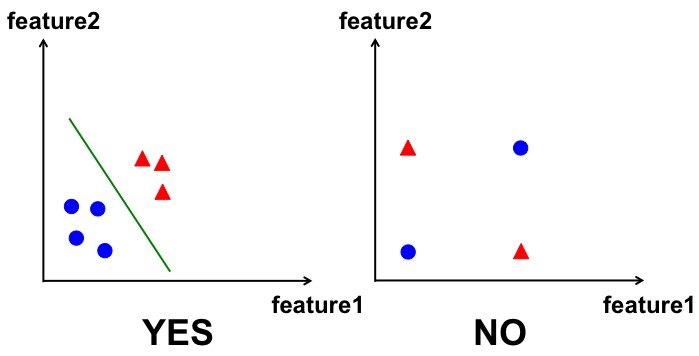
\includegraphics[width=.6\textwidth]{figures/image1.jpg}\\
    Source: http://qingkaikong.blogspot.com
\end{center}

\noindent However, consider the situation on the right of this figure. Is it possible to draw a linear decision boundary which separates the red triangles from the blue dots? We cannot; with as few as four points, it can become impossible to draw a linear decison boundary which separates the points into their respective classes. We refer to data which can be separated by a linear decision boundary as \textit{linearly separable}. As we will see, the perceptron algorithm will only converge to a solution if the underlying data is linearly separable; if it is not, the algorithm will run forever, never converging to a solution. This issue is addressed by other methods such as the \textit{soft-margin support vector machine} (a.k.a soft SVM), which simply finds a good-enough linear decision boundary; this model is not presented here but is discussed in CS 189. \\

\noindent In the case of 2D datapoints, an easy method for determining if the data is linearly separable is to try and draw an oval around all the points of each class; if you cannot draw a convex shape around each class without the shapes overlapping, the data is not linearly separable. Additionally, note that when using the threshold function as a binary classifier, the decision boundary will always be linear and one dimension lower than the data. That is to say, if our data is one-dimensional, our decision boundary will be a point; if our data is two-dimensional, as in this example, our decision boundary will be a line; if our data is three-dimensional, our decision boundary will be a plane; and so on. Other methods can be used to learn more complex decision boundaries, and if time permits we may touch on a few of these at the end of the class. Finally, the choice of how to assign new points which land exactly on the decision boundary is arbitrary; however, if our datapoints are samples from a continuous probability distribution, the probability of new data landing exactly on the boundary is infinitesimal, and so this is not generally an issue in practice. \\

\noindent We now introduce the perceptron algorithm for learning the decision boundary. The algorithm introduces one new parameter, the \textit{learning rate}; this is known as a \textit{hyperparameter}, as it is set by the user of the algorithm and not learned by the algorithm like the other parameters. It is as follows:
\begin{enumerate}[label=\arabic*.]
\item Initialize the weights to zero: $\mathbf{w}^0 = \mathbf{0}$, $b^0 = 0$.
\item For each datapoint $\mathbf{x}_j$ in the training set, perform the following weight update:
	  \begin{enumerate}[label=(\alph*)]
	  \item Calculate the current output for this datapoint: $y_j^t = (\mathbf{w}^t)^{\top}\mathbf{x}_j + b^t$
	  \item Update the weights: $w_i^{t+1} = w_i^t + r(\delta_j - y_j^t)x_{ji}$, $b^{t+1} = b^t + r(\delta_j - y_j^t)$ \\
	  Note that $w_i^t$ is the $i-$th element of the weight vector at time $t$, $x_{ji}$ is the $i-$th element of the datapoint $\mathbf{x}_j$, $\delta_j$ is 1 if $\mathbf{x}_j$ is in class A and 0 if it is in class B, and $r$ is the learning rate.
	  \end{enumerate}
\item Repeat step 2 until convergence.
\end{enumerate}

\noindent This algorithm is guaranteed to converge if the underlying data is linearly separable. However, if the underlying data is not linearly separable, then the $(\delta_j - y_j^t)$ term in the weight update will never be zero for every training point (as we won't be able to properly classify every training point), and so the weights will never converge. Additionally, if the data is linearly separable, the perceptron algorithm will converge as soon as it finds some working decision boundary; there is no guarantee that this decision boundary will generalize well to new data. For these reasons, the perceptron algorithm is rarely used in practice; unless we know prior to training that our underlying data is linearly separable, the algorithm is useless, and so it is preferable to use a model which does not have this assumption to solve binary classification problems (such as the aforementioned soft SVM). Nonetheless, the perceptron algorithm was an important milestone in the early history of artificial intelligence research, and as good a starting point as any as an example of algorithmic learning. 

\end{document}
